% mainfile: ../../../../master.tex
\subsection{DNA quantification with Qubit\texttrademark~ DNA BR Assay Kit}
% The part of the label after the colon must match the file name. Otherwise,
% conditional compilation based on task labels does NOT work.
\label{task:20180313_cj1}
\tags{lab,qnt,dna}
\authors{cj}
%\files{}
%\persons{}

\sidenote{Qubit\texttrademark~ DNA BR Assay Kit \texttt{LOT:\#1835789} opened by Elísabet on 20170815.}

\begin{figure}[H] % position of the figure 
    \centering
    \caption{Illustration for the Qubit\texttrademark~ DNA BR assay}
    \label{fig:20180313_Qubit_dsDNA_BR}
    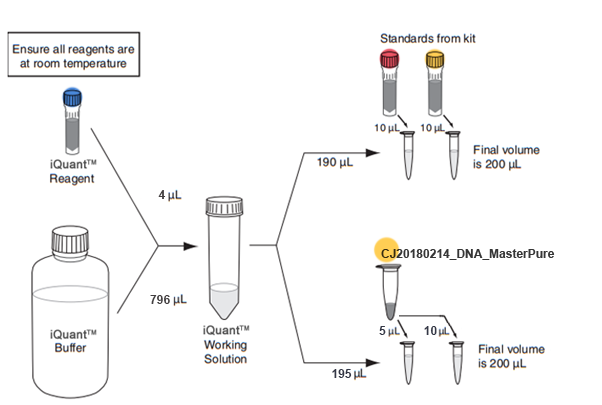
\includegraphics[width=0.8\textwidth]{graphics/schemas/20180215_Qubit_dsDNA_BR.png}
\end{figure}
\comment{It is exactly the same as what was done on the 20180215.}

For the Qubit\texttrademark~ DNA BR Assay, I consider that I have 4 samples: the two standards and one DNA sample that I will measure twice, once using 5~\uL and once using 10~\uL.

Also, I repeat the measure three times. The first time, I use the old calibration. The second time, I re-calibrate the spectrophotometer with the standards prepared by myself.

Because I received a new Qubit\texttrademark~ DNA BR assay kit last week, I want to make sure the measurments are consistent. So today, I will quantify the DNA with the old kit (\texttt{LOT:\#1835789}) and then with the new one (\texttt{LOT:\#1927400}). Measurments obtained with the old kit are presented in table \ref{tab:20180313_nuc_acid_qnt} and  Measurments obtained with the new kit are presented in table \ref{tab:20180313_nuc_acid_qnt_new_kit}. It seems that the results are fairly consistent and therefore I can \textit{trust} the new kit. 

\begin{table}[H]
\caption{Total DNA quantities in samples measured with Qubit\texttrademark~ DNA BR Assay Kit}
\label{tab:20180313_nuc_acid_qnt}
\centering
\begin{tabular}{l r r r r}
\toprule
Sample ID & \textmu g/mL & $V_f$ (mL) & m (\textmu g) & m (ng) \\ \midrule
\texttt{CJ20180313\_DNA\_MP\_5} & 20.0 & 0.018 & 0.360 & 360.0 \\
\texttt{CJ20180313\_DNA\_MP\_10} & 22.7 & 0.018 & 0.408 & 408.6 \\
\midrule
\texttt{CJ20180313\_DNA\_MP\_5} & 14.8 & 0.018 & 0.266 & 266.4 \\
\texttt{CJ20180313\_DNA\_MP\_10} & 16.1 & 0.018 & 0.289 & 289.8 \\
\midrule
\texttt{CJ20180313\_DNA\_MP\_5} & 15.3 & 0.018 & 0.275 & 275.4 \\
\texttt{CJ20180313\_DNA\_MP\_10} & 16.2 & 0.018 & 0.291 & 291.6 \\
\bottomrule
\end{tabular}
\end{table}

\sidenote{Qubit\texttrademark~ DNA BR Assay Kit \texttt{LOT:\#1927400} opened by myself today.}
\begin{table}[H]
\caption{Total DNA quantities in samples measured with Qubit\texttrademark~ DNA BR Assay Kit recently received}
\label{tab:20180313_nuc_acid_qnt_new_kit}
\centering
\begin{tabular}{l r r r r}
\toprule
Sample ID & \textmu g/mL & $V_f$ (mL) & m (\textmu g) & m (ng) \\ \midrule
\texttt{CJ20180313\_DNA\_MP\_5} & 8.15 & 0.018 & 0.146 & 146.7 \\
\texttt{CJ20180313\_DNA\_MP\_10} & 8.94 & 0.018 & 0.160 & 160.9 \\
\midrule
\texttt{CJ20180313\_DNA\_MP\_5} & 17.5 & 0.018 & 0.315 & 315.0 \\
\texttt{CJ20180313\_DNA\_MP\_10} & 18.4 & 0.018 & 0.331 & 331.2 \\
\midrule
\texttt{CJ20180313\_DNA\_MP\_5} & 17.0 & 0.018 & 0.306 & 306.0 \\
\texttt{CJ20180313\_DNA\_MP\_10} & 18.3 & 0.018 & 0.329 & 329.4 \\
\bottomrule
\end{tabular}
\end{table}

In table \ref{tab:20180301_nuc_acid_qnt}, the quantities of DNA are calculted based on the volume left: I know resuspended the DNA 50~\uL of Tris HCl buffer, which means I was able to obtain at least 850 ng of DNA. Then I used 2~\uL for the NanoDrop\cR measurments and finally I use 5~\uL and 10~\uL twice for the Qubit\texttrademark~ assays. Which means the volume left us 18~\uL in which I have - at least - 300 ng of DNA left.
